\graphicspath{{./fig_Eq/}}

\section{支配方程式}
\label{sec:basic eqs}
流体の密度変化\index{みつどへんか@密度変化}は圧力や温度の変化により生じる.代表的な流速が音速に比べてかなり低い場合,流体の挙動は圧縮性,つまり密度変化による媒質の弾性の影響が小さいと近似でき,非圧縮性流体として扱うことができる.
一方,代表流速が音速よりかなり低い場合でも,弾性の影響を考慮しなければならない場合もある.この場合,対象とする流れの現象を考慮して基礎方程式を適切にモデル化して解く.モデル化のレベルによって,下記のようなバリエーションが考えられる.

\begin{itemize}
\item[1)] 圧縮性方程式を近似せずに扱う~\cite{kotake:94:handbook}
\item[2)] 弾性の影響を質量保存則のみに適用し,運動量に与える密度変化を省略する
\item[3)] 温度変化によって生じる密度変化を運動方程式の外力としてモデル化する
\item[4)] 完全に非圧縮性流体として扱う
\end{itemize}
ここでは,2)-4) の定式化を説明する.

\subsection{非圧縮性流体}
解析対象とする流れの特徴を以下のように仮定し,支配方程式を記述する.

\begin{itemize}
\item 流れの速度が音速に比べて十分に低く,流れの運動に対する圧縮性の影響は小さいと仮定し,流れを非圧縮性として取り扱う.
\item 温度場の代表的な温度差スケールが$30\ {}^\circ\mathrm{C}$以下で,密度変化が小さいと仮定すると,密度変化が質量保存則へ与える影響は小さい.密度変化が流れの運動に及ぼす影響をBoussinesq近似\index{ぶしねきんじ@Boussinesq近似}\index{Boussinesq}によりモデル化する.
\end{itemize}

支配方程式として,非圧縮性流れに対する質量保存則\textbf{(\ref{eq:continuity eq})},運動量保存則\textbf{(\ref{eq:NS eq})},エネルギー保存則\textbf{(\ref{eq:energy eq})}を用いる.
$\delta$はクロネッカーのデルタで重力方向 (i=3) のときに浮力が作用する.
ここで,プライム$[{}^{\prime}]$は有次元量を表す.物性値など有次元であることが明らかなものにはプライムは付けていない.

\begin{equation}
\frac{ \partial{{u}_{i}}^{\prime} }{ \partial{{x}_{i}}^{\prime} }\,{=}\,{0}
\label{eq:continuity eq}
\end{equation}

\begin{equation}
\rho^{\prime} \frac{\partial{{u}_{i}}^{\prime}}{\partial{t}^{\prime}} + \rho^{\prime} \frac{\partial}{\partial{{x}_{j}}^{\prime}} \left \{ \,\left( u_j^\prime - u_j^{\,g\,\prime} \right) \,u_i^\prime\,\right \}
\,{=}\,
- \frac{\partial{P}^{\prime}}{\partial{{x}_{i}}^{\prime}} + \frac{\partial}{\partial{{x}_{j}}^{\prime}} \left[ {\mu\left({ \frac{\partial{{u}_{i}}^{\prime}}{\partial{{x}_{j}}^{\prime}} + \frac{\partial{{u}_{j}}^{\prime}}{\partial{{x}_{i}}^{\prime}}} \right)} \right] - \rho^{\prime} {g}{\delta}_{i3}
\label{eq:NS eq}
\end{equation}

\begin{equation}
\rho^\prime C_p \left[ \frac{\partial \theta^\prime}{\partial t^\prime} + \frac{\partial}{\partial x_i^\prime} \left\{ \, \left( u_i^\prime - u_i^{\,g\,\prime} \right) \theta^\prime \, \right\} \right] 
\,{=}\,
\frac{D{P}^{\prime}}{D{t}^{\prime}} + \frac{\partial}{\partial{{x}_{i}}^{\prime}} \left( {\lambda \frac{\partial{\theta}^{\prime}}{\partial{{x}_{i}}^{\prime}}} \right) + \mu\Phi + {Q}^{\prime}
\label{eq:energy eq}
\end{equation}

\vspace{1.0cm}
\begin{center}
\begin{tabular}{lll}
$\rho^{\prime}$ &  $[kg\,/\,m^3]$ & density \\
$P^{\prime}$ & $[Pa]$ & pressure \\
${C}_{p}$ & $[J\,/\,(kg\,K)]$ & specific heat at constant pressure \\
$\theta^{\prime}$ & $[K]$ & temperature \\
$\lambda$ & $[W\,/\,(m\,K)]$ & heat conductivity \\
${{u}_{j}}^{\prime}$ & $[m\,/\,s]$ & velocity components \\
$u_j^{\,g\,\prime}$ & $[m\,/\,s]$ & velocity components of a grid point \\
${{x}_{j}}^{\prime}$ & $[m]$ & coordinate axis\\
$t^{\prime}$ & $[s]$ & time\\
$\mu$ & $[Pa\,s]$ & viscosity\\
$g$ & $[m\,/\,s^2]$ & gravitational acceleration\\
$\Phi$ & $[1/s^{2}]$ & dissipation function\\
$Q^{\prime}$ & $[W\,/\,m^3]$ & heat source\\
\end{tabular}
\end{center}
\vspace{1.0cm}

\noindent \textbf{式(\ref{eq:NS eq})}は形式的にALE(Arbitrary Lagrangian and Eulerian)\index{ALE}で書かれているが,速度$u_j^{\,g\,\prime}$で移動する格子系での保存則を表現している.格子点を固定($u_j^{\,g\,\prime}=0$)すればEuler表現,流体粒子と一緒に移動($u_j^{\,g\,\prime}=u_j^\prime$)させればLagrangian表現となる.ここでは,並進や回転などの任意の格子移動速度を与えるために$u_j^{\,g\,\prime}$を利用する.\\

一様で平衡な状態においては,密度は圧力と温度の関数となる.理想気体\index{りそうきたい@理想気体}の場合には,$\mathcal{R}$\,(8.314472 $[J\,/\,(mol\,K)]$ を気体定数~\cite{codataR}\footnote{気体定数の値はCODATA(科学技術データ委員会)の2002年の勧告で,それ以前から変更になっている.}とすると\textbf{式(\ref{eq:state eq})}により表される.

\begin{equation}
{P}^{\prime}\,{=}\,\rho^{\prime}\,\mathcal{R}\,\mathrm{\theta}^{\prime}
\label{eq:state eq}
\end{equation}

\noindent 平衡状態0からのずれが小さく変化が線形であると仮定すると,テーラー展開から

\begin{equation}
\rho^{\prime}
\, = \,
{\rho_{0}}^{\prime} + {\left( { \frac{\partial \rho^{\prime}} {\partial \theta^{\prime}} } \right)}_{0} \left( \theta^{\prime} - {\theta_{0}}^{\prime} \right) + {\left( { \frac{\partial\rho^{\prime}}{\partial{P}^{\prime}} } \right)}_{0} \left( { P^{\prime} - {P_{0}}^{\prime} } \right)
\label{eq:Taylor exp:density}
\end{equation}

\noindent ここで,体積膨張率\index{たいせきぼうちょうりつ@体積膨張率}を次式で定義すると,

\begin{equation}
{\mathrm{\beta}}_{0}
\,{=}\,
{-}\frac{1}{{{\rho}_{0}}^{\prime}} {\left( {\frac{\partial{\rho}^{\prime}}{\partial{\theta}^{\prime}}} \right) }_{0}
\end{equation}

\noindent 理想気体の場合には,

\begin{equation}
{\mathrm{\beta}}_{0}\,{=}\,\frac{1}{{\theta_{0}}^{\prime}}
\end{equation}

\noindent となる.\textbf{(\ref{eq:Taylor exp:density})}の右辺第三項は音速の2乗に反比例するので省略でき,最終的に次のようになる.

\begin{equation}
\rho^{\prime}
\,{=}\,
{\rho_{0}}^{\prime} - {\rho_{0}}^{\prime} {\mathrm{\beta}}_{0} \left({ \theta^{\prime} - {\theta_{0}}^{\prime} }\right)
\label{eq:Boussinesq model}
\end{equation}

\noindent \textbf{式(\ref{eq:Boussinesq model})}は,基準状態$\,0\,$を基にして密度変化\index{みつどへんか@密度変化}を温度変化によって表すBoussinesq近似\index{ぶしねきんじ@Boussinesq近似}\index{Boussinesq}モデルである.\\

さて,重力下にある静止流体では下層にある流体ほど圧力が高い.三次元の z 方向(i=3)を鉛直方向にとると,Navier-Stokes方程式\textbf{(式\ref{eq:NS eq})}の右辺は,状態$\,0\,$のとき,

\begin{equation}
{-}\frac{\partial P^{\prime}}{\partial{{x}_{i}}^{\prime}} - {\rho_{0}}^{\prime}{g}
\, =\, 
{-}\frac{\partial}{\partial{z}^{\prime}} \left({ P^{\prime} + {\rho_{0}}^{\prime} g {z}^{\prime} }\right) 
\,{=}\,
{-}\frac{\partial{\tilde{p}}^{\prime}}{\partial{z}^{\prime}}
\end{equation}

\noindent である.重力ポテンシャル\index{じゅうりょくぽてんしゃる@重力ポテンシャル}の影響を加えた新しい定義の圧力を導入し,支配方程式を表すと,\textbf{式(\ref{eq:NS eq})}は以下のようになる.

\begin{equation}
{\tilde{p}}^{\prime} \,{=}\, {P}^{\prime} {+} {\rho_{0}}^{\prime} g {z}^{\prime}
\end{equation}

\begin{equation}
\frac{\partial{{u}_{i}}^{\prime}} {\partial{t}^{\prime}} + \frac{\partial}{\partial{{x}_{j}}^{\prime}} \left \{ \,\left( u_j^\prime - u_j^{\,g\,\prime} \right) \, u_i^\prime \, \right \}
\,{=}\,
- \frac{\partial{p}^{\prime}}{\partial{{x}_{i}}^{\prime}} + \frac{\partial}{\partial{{x}_{j}}^{\prime}} \left[{ \mathrm{\nu}\left({\frac{\partial{{u}_{i}}^{\prime}}{\partial{{x}_{j}}^{\prime}} + \frac{\partial{{u}_{j}}^{\prime}}{\partial{{x}_{i}}^{\prime}} }\right) }\right] - \left({ \theta^{\prime} - {\theta_{0}}^{\prime} }\right) \beta_{0} g \delta_{i3}
\label{eq:NS eq2}
\end{equation}

\vspace{5mm}
\noindent また,低マッハ数\index{ていまっはすう@低マッハ数}を仮定すると,散逸関数$\Phi$は$M^2$に比例するので,その寄与は小さいとしてよい.圧力の全微分の項の影響も小さいとすると,\textbf{式(\ref{eq:energy eq})}は,

\begin{equation}
\frac{\partial \theta^{\prime}}{\partial{t}^{\prime}} + \frac{\partial}{\partial{{x}_{i}}^{\prime}} \left\{ \, \left( u_i^\prime - u_i^{\,g\,\prime} \right) \, \theta^\prime \, \right \}
\,{=}\, 
\frac{\partial}{\partial{{x}_{i}}^{\prime}} \left({ \mathrm{\alpha} \frac{\partial \theta^{\prime}}{\partial{{x}_{i}}^{\prime}} }\right) + \frac{Q^{\prime}}{\rho^{\prime}{C}_{p}}
\label{eq:thermal transport eq}
\end{equation}

\noindent ここで$\alpha$は温度拡散係数\index{おんどかくさんけいすう@温度拡散係数}で$[m^2/s]$の単位をもつ.

\begin{equation}
\qquad \left.
\begin{array}{ll}
\vspace{2mm}
\alpha\,=\, \displaystyle{ \frac{\lambda}{\rho^{\prime} C_{p}} } & [m^2/s]\\
\vspace{2mm}
\nu\,=\, \displaystyle{ \frac{\mu}{\rho^{\prime}} } & [m^2s]\\
\vspace{2mm}
p\,=\, \displaystyle{ \frac{{\tilde{p}}^{\prime}}{{\rho_{0}}^{\prime}} } & [m^2/s^2]
\end{array} \quad \right\}
\label{eq:thermal transport eq2}
\end{equation}

\noindent とおいた.温度拡散係数$\alpha$が一定,さらに定常の場合には下記のようになる.

\begin{equation}
\frac{\partial \theta^{\prime}}{\partial{t}^{\prime}} + \frac{\partial}{\partial{{x}_{i}}^{\prime}} \left\{ \, \left( u_i^\prime - u_i^{\,g\,\prime} \right) \, \theta^\prime \, \right \} 
\,{=}\,
\mathrm{\alpha} \frac{\partial}{\partial{{x}_{i}}^{\prime}} \left({ \frac{\partial \theta^{\prime}}{\partial{{x}_{i}}^{\prime}} }\right) + \frac{Q^{\prime}} {\rho^{\prime} {C}_{p}}
\label{thermal transport eq:const alpha}
\end{equation}

\begin{equation}
\frac{\partial}{\partial{{x}_{i}}^{\prime}} \left\{ \, \left( u_i^\prime - u_i^{\,g\,\prime} \right) \, \theta^\prime \, \right \}  
\,{=}\,
\mathrm{\alpha} \frac{\partial}{\partial{{x}_{i}}^{\prime}} \left({ \frac{\partial \theta^{\prime}}{\partial{{x}_{i}}^{\prime}} }\right) + \frac{Q^{\prime}}{\rho^{\prime} {C}_{p}}
\label{eq:steady thermal transport eq:const alpha}
\end{equation}

%
\section{無次元化}
\label{sec:non dimensionalize}
代表速度$u_0^\prime$, 代表長さ$L^\prime$, 代表温度スケール$\Delta \theta^\prime$と基準温度$\theta_0^\prime$で\textbf{式(\ref{eq:continuity eq})}, \textbf{(\ref{eq:NS eq2})}, \textbf{(\ref{eq:thermal transport eq})}を無次元化\index{むじげんか@無次元化}する.

\begin{equation}
\left.{ \begin{array}{l}
\vspace{2mm}
{u \,{=}\, \displaystyle{ \frac{ u^{\prime} } { {u_{0}}^{\prime}} } }\\
\vspace{2mm}
x \,{=}\, \displaystyle{ \frac{x^{\prime}}{L^{\prime}} }\\
\vspace{2mm}
p \,=\, \displaystyle{ \frac{p^\prime - {p_0}^\prime}{\rho^\prime {u_0^\prime}^2} }\\
\vspace{2mm}
\theta \,{=}\, \displaystyle{ \frac{\theta^{\prime} - {\theta_{0}}^{\prime}}{\Delta \theta^{\prime}} }
\end{array}\quad }\right\}
\label{eq:non dimensional basis}
\end{equation}

%
\subsection{強制対流と自然対流}
\label{sec:natural_convection}
以下の\textbf{式(\ref{eq:continuity eq:ND})}--\textbf{(\ref{eq:thermal transport eq:ND})}は,単一成分の熱流動を表す.

\begin{equation}
\frac{\partial{u}_{i}}{\partial{x}_{i}}\,{=}\,{0}
\label{eq:continuity eq:ND}
\end{equation}

\begin{equation}
\frac{\partial{u}_{i}}{\partial{t}}{+}\frac{\partial}{\partial{x}_{j}} \left\{ \, \left( u_j - u_j^{\,g} \right) \, u_i \, \right\}
\,{=}\,
{-}\frac{\partial{p}}{\partial{x}_{i}}{+}\frac{1}{Re}\frac{\partial}{\partial{x}_{j}}\left({\frac{\partial{u}_{i}}{\partial{x}_{j}}{+}\frac{\partial{u}_{j}}{\partial{x}_{i}}}\right){+}\frac{Gr}{{Re}^{2}}{\mathrm{\delta}}_{i3}\mathrm{\theta}
\label{eq:NS eq:ND}
\end{equation}

\begin{equation}
\frac{\partial\mathrm{\theta}}{\partial{t}}{+}\frac{\partial}{\partial{x}_{i}} \left\{ \, \left( u_i - u_i^{\,g} \right) \, \mathrm{\theta} \, \right\}
\,{=}\,
\frac{1}{Pe}\frac{\partial}{\partial{x}_{i}}\frac{\partial\mathrm{\theta}}{\partial{x}_{i}}{+}\mathrm{\Theta}
\label{eq:thermal transport eq:ND}
\end{equation}

\begin{equation}
\left.{\begin{array}{l}
\vspace{2mm}
{{Re}\,{=}\,\frac{\displaystyle {{u}'}_{0}{L}'}{\displaystyle \mathrm{\nu}}}\\
\vspace{2mm}
{{Pr}\,{=}\,\frac{\displaystyle \mathrm{\mu}{C}_{p}}{\displaystyle \mathrm{\lambda}}\,{=}\,\frac{\displaystyle \mathrm{\nu}}{\displaystyle \mathrm{\alpha}}}\\
\vspace{2mm}
{{Gr}\,{=}\,\frac{\displaystyle {g}\mathrm{\beta}\mathrm{\Delta}{\mathrm{\theta}}'{{L}'}^{3}}{\displaystyle {\mathrm{\nu}}^{2}}}\\
\vspace{2mm}
{{Ra}\,{=}\,{Pr}\mathrm{\cdot}{Gr}}\\
\vspace{2mm}
{{Pe}\,{=}\,{Pr}\mathrm{\cdot}{Re}}\\
\vspace{2mm}
{\mathrm{\Theta}\,{=}\,\frac{\displaystyle Q^{\prime}}{\displaystyle {\mathrm{\rho}}'{C}_{p}}\frac{\displaystyle {L}'}{\displaystyle {{u}'}_{0}\mathrm{\Delta}{\mathrm{\theta}}'}}
\end{array}\quad }\right\}
\label{eq:ND definition}
\end{equation}

\noindent ここで,
\vspace{1.0cm}
\begin{center}
\begin{tabular}{lll}
$Pr$ & Prandtl数 & 粘性と熱の拡散率の比\\
$Re$ & Reynolds数 & 慣性力と粘性力の比\\
$Gr$ & Grashof数 & 浮力と粘性力の比\\
$Ra$ & Rayleigh数 & 不安定性のパラメータ\\
$Pe$ & Peclet数 & 対流と熱伝達のエネルギー輸送の比\\
$\Theta$ & - & 無次元の温度変化率\\
\end{tabular}
\end{center}
\vspace{1.0cm}

\noindent \textbf{式(\ref{eq:NS eq:ND})}は強制対流と自然対流を表現している.右辺第三項は自然対流と強制対流の比を表している.つまり,$Gr/Re^2 \gg 1$の場合には自然対流が支配的で,$Gr/Re^2 \ll 1$の場合には強制対流が支配的となる.$Gr = 0$つまり温度差が無い場合には純強制対流である.
一方,$Gr/Re^2 \rightarrow \infty$の場合には純自然対流で,流れは浮力によって駆動されるため代表速度が自明ではない.
また,$Gr > 10^9$となるような流れは非定常性が強くなる.

\subsection{自然対流のスケールアナリシス}

純自然対流の場合の代表流速をスケールアナリシスから推測する\cite{nakayama:02:netsuryuutai}.
自然対流の場合には流れを駆動する支配要因が熱拡散であり,対流の影響は小さいと考えられるので,温度境界層と粘性境界層の厚さが同程度と見積もられる.
ところで,$Pr$数が大きな流体の場合には粘性が支配的なので,\textbf{式(\ref{eq:NS eq:ND})}において,粘性項と浮力項のオーダーが等しい.
一方,低$Pr$数流体の場合には慣性力が支配的となるので,慣性項と浮力項のオーダーが等しくなる.
これらをまとめると,

\begin{equation}
\left.
\begin{array}{llll}
\vspace{1mm}
\displaystyle{ \frac{Gr}{Re^2} \delta_{i3} \theta } & \sim & 
\displaystyle{ \frac{1}{Re} \frac{\partial}{\partial x_j} \left({ \frac{\partial u_i}{\partial x_j} + \frac{\partial u_j}{\partial x_i} }\right) } &
(Pr \, \gg \, 1)\\
\displaystyle{ \frac{Gr}{Re^2} \delta_{i3} \theta } & \sim & 
\displaystyle{ \frac{\partial}{\partial x_j} \left({ u_i u_j }\right) } & (Pr \, \ll \, 1)
\end{array} \qquad \right \}
\label{eq:scaling natural 1}
\end{equation}

\noindent $Pr$数が小さい場合は\textbf{式(\ref{eq:scaling natural 1})}から,

\begin{equation}
u_{\mathit 0}^\prime \, = \, \sqrt{g \beta \Delta \theta^\prime L^\prime}
\label{eq:scaling natural u_ref}
\end{equation}

\noindent と見積もることができる.したがって,自然対流の場合の代表速度は\textbf{式(\ref{eq:scaling natural u_ref})}の関係を用いて見積もり,代表速度パラメータとして与える.自然対流と強制対流が共存する共存対流の場合には,各々の代表スケールの平均値や大きい方の値を代表速度とする.


\subsection{熱流動計算の支配方程式とパラメータ}
各流動現象の支配方程式に対する入力パラメータ(Kind\_Of\_Solver, Buoyancy)と支配方程式の関係を\textbf{表\ref{tbl:thermal mode}}にまとめる\footnote{共役熱移動と固体熱伝導についての詳細は,\ref{chpt:m_medium}章で説明する.}.パラメータは全て有次元で入力\footnote{純強制対流の場合のみ無次元パラメータにも対応している.}\ するが,標準出力には対応する無次元数も出力する.\\

\begin{table}[htdp]
\small
\caption{支配方程式と熱対流計算のパラメータ指定の関係}
\begin{center}
\begin{tabular}{lll} \toprule
支配方程式 & Kind\_Of\_Solver & Buoyancy\\ \midrule
純強制対流 & Flow\_Only & -\\
熱対流(浮力なし)& Thermal\_Flow & No\_Buoyancy\\
熱対流(浮力あり)& Thermal\_Flow & Boussinesq\\
%& & Low\_Mach\\
自然対流 & Thermal\_Flow\_Natural & Boussinesq\\
%& & Low\_Mach\\
固体熱伝導 & Solid\_Conduction & -\\ \bottomrule
%共役熱移動 & Conjugate\_Heat\_Transfer & Boussinesq\\ 
%& & Low\_Mach\\ \bottomrule
\end{tabular}
\end{center}
\label{tbl:thermal mode}
\end{table}


\subsubsection{純強制対流}
\begin{indentation}{5zw}{0zw}
\noindent \textbf{式(\ref{eq:NS eq:ND})}においては$\,Gr=0\,$なので$\,Re\,$が支配パラメータとなる.
無次元化のスケーリングは,$\,{u_{0}}^{\prime},\,L^{\prime},\,\nu,\,\,\alpha\,(\,=\lambda / \rho^{\prime} C_{p})\,$を与える.\\

\end{indentation}

\subsubsection{熱対流}
\begin{indentation}{5zw}{0zw}
\paragraph{浮力の効果を考慮しない場合}
\noindent \textbf{式(\ref{eq:NS eq:ND})}において,純強制対流と同じく$\,Gr=0\,$である.\textbf{式(\ref{eq:thermal transport eq:ND})}では$Pe\,$が支配パラメータとなる.
無次元化のスケーリングは,$\,{u_{0}}^{\prime},\,L^{\prime},\,\nu,\,\,\alpha\,(\,=\lambda / \rho^{\prime} C_{p})\,$を与える.\\
\paragraph{浮力の効果を考慮する場合}
\textbf{式(\ref{eq:NS eq:ND})}では$\,Gr,\,Re\,$が,\textbf{式(\ref{eq:thermal transport eq:ND})}では$\,Pe\,$が支配パラメータとなる.
無次元化のスケーリングは,$\,{u_{0}}^{\prime},\,L^{\prime},\,\Delta\theta^{\prime},\,\beta,\,g,\,\nu,\,\alpha,\,Pr\,$を与える.\\
\end{indentation}

\subsubsection{純自然対流}
\begin{indentation}{5zw}{0zw}
\noindent 浮力の効果を考慮した熱対流と同じである.ただし,${u_{0}}^{\prime}$は自明でないので,\textbf{式(\ref{eq:scaling natural u_ref})}により適切に見積る点に注意する.\\
\end{indentation}

\subsubsection{固体熱伝導}
\begin{indentation}{5zw}{0zw}
\noindent \textbf{式(\ref{eq:thermal transport eq:ND})}の形式で$\,Pe\,$が支配パラメータとなる.ただし,対流項の寄与はゼロである.
無次元化のスケーリングは,$\,L^{\prime},\,\Delta \theta^{\prime},\,\alpha,\,$を与え,$\,{u_{0}}^{\prime}$には\textbf{式(\ref{eq:velocity scale in natural convection})}を用いる.\\
\end{indentation}

\subsubsection{共役熱移動}
\begin{indentation}{5zw}{0zw}
\noindent 共役熱移動は,固体中の熱移動と流体中の熱流動を同時に扱うので,必然的に多媒質の熱移動問題となる.熱流動は浮力効果を考慮している.
%式(\ref{eq:NS eq:ND})では$\,Gr,\,Re$,式(\ref{thermal transport eq:ND})では$Pe\,$が支配パラメータとなる.無次元化のスケーリングは,$\,L^{\prime},\,\Delta\theta^{\prime},\,\beta,\,g,\,\nu,\,\alpha,\,Pr,\,$を与え,適切な$\,{u_{0}}^{\prime}$を用いる.\\
\end{indentation}



%
\section{解法アルゴリズム}
\label{sec:Algorithm NS}
この節では前節の支配方程式に対して,非圧縮性流体の解法に使われる分離解法\index{ぶんりかいほう@分離解法}を適用し,有限体積法で離散化する.

\subsection{Fractional Step法}
\label{sec:fractional step}
非圧縮性のNavier-Stokes方程式\textbf{(\ref{eq:NS eq:ND})}の解法として,Fractional step法\index{Fractional step}を用いる.これは,任意のベクトル場が非回転場と湧き出し無しの直交するベクトル場に分解できる性質を利用して,二つのベクトルの和をとることにより解を求める分離解法である.

離散式のコーディングポリシーとして,各セル単位で計算を進めていく.保存的な支配方程式を解くのでセル界面の流束ベースの評価が素直で演算量も少なくなるが,コロケートでは固体面や境界面の処理を考える上でセル単位毎の方が計算処理がしやすい.

%
\subsubsection{Euler Explicit}
\begin{indentation}{5zw}{0zw}
一次精度の時間進行法である.

\paragraph{Navier-Stokes equations} $\mbox{}$\\
\textbf{式(\ref{eq:NS eq:ND})}の対流項と粘性項をそれぞれ$C_i,\,D_i$,浮力項を外力$f_i$で表すと,

\begin{equation}
\left.
\begin{array}{l}
\vspace{2mm}
\displaystyle{ \frac{\partial u_i}{\partial t} + C_i \,=\, - \frac{\partial p}{\partial x_i} + D_i + f_i } \\
\vspace{2mm}
\qquad \displaystyle{ C_i \,=\, \frac{\partial}{\partial x_j} \left\{ \, \left( u_j - u_j^{\,g} \right) \, u_i \, \right\} } \\
\vspace{2mm}
\qquad \displaystyle{ D_i \,=\, \frac{1}{Re}\frac{\partial}{\partial x_j} \left( \frac{\partial u_i}{\partial x_j} + \frac{\partial u_j}{\partial x_i} \right) } \\
\vspace{2mm}
\qquad \displaystyle{ f_i \,=\, \frac{Gr}{{Re}^2} \delta_{i3} \theta } \\
\end{array} \quad \right \}
\label{eq:NS eq CDf}
\end{equation}

\noindent 疑似ベクトルの予測式は,
\begin{equation}
u_i^{\,*} \,=\, u_i^{\,n} + \Delta t \left( D_i^{\,n} - C_i^{\,n} + f_i^{\,n} \right)
\label{eq:pseudo vector EE}
\end{equation}

\noindent 連続の式による拘束条件から,圧力のPoisson方程式は,
\begin{equation}
\frac{\partial}{\partial x_i} {\frac{\partial p}{\partial x_i}}^{n+1}
\,=\,
\frac{1}{\Delta t} {\frac{\partial \bar{u}_i}{\partial x_i}}^* \vspace{1mm}
\label{eq:Poisson eq}
\end{equation}

\noindent 圧力ポテンシャルによるセルセンターとスタガード位置の速度ベクトルの修正式は,
\begin{equation}
u_i^{\,n+1} \,=\, u_i^{\,*} - \Delta t {\frac{\partial p}{\partial x_i}}^{n+1}
\label{eq:Pressure correction CC}
\end{equation}

\begin{equation}
u_{i,\,face}^{\,n+1} \,=\, \bar{u}_{i,\,face}^{\,*} - \Delta t {\frac{\partial p}{\partial x_i}}^{n+1}
\label{eq:Pressure correction CF}
\end{equation}

\paragraph{Thermal transport equation} $\mbox{}$\\
\textbf{式(\ref{eq:thermal transport eq:ND})}の移流項と拡散項をそれぞれ$Cs_i,\,Ds_i$で表すと,

\begin{equation}
\left.
\begin{array}{l} 
\vspace{2mm}
\displaystyle { \frac{\partial \theta}{\partial t} + Cs_i \,=\, Ds_i + \Theta } \\
\vspace{2mm}
\qquad \displaystyle{ Cs_i \,=\, \frac{\partial}{\partial x_i} \left\{ \, \left( u_i - u_i^{\,g} \right) \, \theta \, \right\} } \\
\vspace{2mm}
\qquad \displaystyle{ Ds_i \,=\, \frac{1}{Pe}\frac{\partial}{\partial x_i} \frac{\partial \theta}{\partial x_i} } \\
\end{array} \quad \right \}
\label{eq:thermal transport eqs}
\end{equation}

\begin{equation}
\theta^{\,n+1} \,=\, \theta^{\,n} + \Delta t \left( Ds_i^{\,n} - Cs_i^{\,n} + \Theta^{\,n} \right)
\label{eq:thermal transport EE}
\end{equation}

\end{indentation}

%
\subsubsection{Adams-Bashforth}
\begin{indentation}{5zw}{0zw}
二次精度ではあるが,安定条件が厳しい.

\paragraph{Navier-Stokes equations}
\begin{equation}
u_i^{\,*} \,=\, u_i^{\,n} + \Delta t \left[ \frac{1}{2} \left\{  3 \left( D_i^{\,n} - C_i^{\,n} \right)
               - \left( D_i^{\,n-1} - C_i^{\,n-1} \right) \, \right\} + \frac{1}{2} \left( 3f_i^{\,n} - f_i^{\,n-1} \right) \, \right]
\label{eq:pseudo vector AB}
\end{equation}

\paragraph{Thermal transport equation}
\begin{equation}
\theta^{\,n+1} \,=\, \theta^{\,n} + \Delta t \left[ \frac{1}{2} \left\{ 3\left( Ds_i^{\,n}- Cs_i^{\,n} \right) - \left( Ds_i^{\,n-1}- Cs_i^{\,n-1} \right) \right\} + \frac{1}{2} \left( 3\Theta^{\,n} -\Theta^{\,n-1} \right) \, \right]
\label{eq:thermal transport AB}
\end{equation}

\end{indentation}

%
\subsubsection{Adams-Bashforth + Crank-Nicolson}
\begin{indentation}{5zw}{0zw}
拡散項に由来する安定条件による時間積分幅の制限を緩和するため,陰解法を導入する.

\paragraph{Navier-Stokes equations}
\begin{equation}
u_i^{\,*} \,=\, u_i^{\,n} + \Delta t \left[ - \frac{1}{2} \left(  3 C_i^{\,n} - C_i^{\,n-1} \right)
               + \frac{1}{2} \left( D_i^{\,n} + D_i^{\,*}  \right) + \frac{1}{2} \left( 3f_i^{\,n} - f_i^{\,n-1} \right) \, \right]
\label{eq:pseudo vector ABCN}
\end{equation}

\noindent 実装は,

\begin{equation}
\left.
\begin{array}{l}
\vspace{2mm}
\displaystyle{ \bar{u}_i \,=\, u_i^{\,n} \,+\, \Delta t \left[ - \frac{1}{2} \left(  3 C_i^{\,n} - C_i^{\,n-1} \right)
+ \frac{1}{2} D_i^{\,n} + \frac{1}{2} \left( 3f_i^{\,n} - f_i^{\,n-1} \right) \, \right] } \\
\vspace{2mm}
\displaystyle{ u_i^* \,=\, \bar{u}_i \,+\, \frac{\Delta t}{2} \bar{D} }\\
\vspace{2mm}
\displaystyle{ u_{\,i,j,k}^* \,=\, \bar{u}_{\,i,j,k} \,+\, \frac{\Delta t}{2\,Re\,h^2} \left( \sum \limits_l {u_{\,l}^*} - 6\,u_{\,i,j,k}^* \right) } \\
\vspace{2mm}
\displaystyle{ \left( 1 + \frac{3\,\Delta t}{Re\,h^2} \right) u_{\,i,j,k}^* \,=\, \bar{u}_{\,i,j,k} + \frac{\Delta t}{2\,Re\,h^2} \sum \limits_l {u_{\,l}^*} } \\
\end{array} \quad \right\}
\label{eq:CN iteration ABCN}
\end{equation}

\paragraph{Thermal transport equation}
\begin{equation}
\theta^{\,n+1} \,=\, \theta^{\,n} + \Delta t \left[ - \frac{1}{2} \left( 3 Cs_i^{\,n} - Cs_i^{\,n-1} \right) + 
\frac{1}{2} \left( Ds_i^{\,n} + Ds_i^{\,n+1}\right) + \frac{1}{2} \left( 3\Theta^{\,n} -\Theta^{\,n-1} \right) \, \right]
\label{eq:thermal transport ABCN}
\end{equation}

\noindent 実装は,

\begin{equation}
\left.
\begin{array}{l}
\vspace{2mm}
\displaystyle{ \bar{\theta} \,=\, \theta^{\,n} + \Delta t \left[ - \frac{1}{2} \left( 3 Cs_i^{\,n} - Cs_i^{\,n-1} \right) + 
\frac{1}{2} Ds_i^{\,n} + \frac{1}{2} \left( 3\Theta^{\,n} -\Theta^{\,n-1} \right) \, \right] } \\
\vspace{2mm}
\displaystyle{ \theta^{\,n+1} \,=\, \bar{\theta} + \frac{\Delta t}{2} Ds_i^{\,n+1} } \\
\vspace{2mm}
\displaystyle{ \theta_{\,i,j,k}^{\,n+1} \,=\, \bar{\theta}_{\,i,j,k} + \frac{\Delta t}{2\,Pe\,h^2} \left( \sum \limits_l {\theta_{\,l}^{\,n+1}} - 6\,\theta_{\,i,j,k}^{\,n+1} \right) } \\
\vspace{2mm}
\displaystyle{ \left( 1 + \frac{3\,\Delta t}{Pe\,h^2} \right) \theta_{\,i,j,k}^{\,n+1} \,=\, \bar{\theta}_{\,i,j,k} + \frac{\Delta t}{2\,Pe\,h^2} \sum \limits_l {\theta_{\,l}^{\,n+1}} } \\
\end{array} \quad \right\}
\label{eq:CN iteration ABCN thermal}
\end{equation}

\end{indentation}

%
\subsubsection{Runge-Kutta + Crank-Nicolson}
\begin{indentation}{5zw}{0zw}
二次精度の時間進行法,対流項には2段階Runge-Kutta法\index{Runge-Kutta},拡散項にはCrank-Nicolson法\index{Crank-Nicolson}を用いる.

\paragraph{1st step : Predictor} $\mbox{}$\\
積分幅を$\Delta t/2$にとりEuler陽解法で時間積分し,n+1/2タイムレベルでの予測値を得る.

\subparagraph{Navier-Stokes equations}

\begin{equation}
u_i^{\,*,\,n+1/2} \,=\, u_i^{\,n} + \frac{\Delta t}{2} \left( D_i^{\,n} - C_i^{\,n} + f_i^{\,n} \right) \vspace{2mm}
\label{eq:pseudo vector RKCN predictor}
\end{equation}

$n+1/2\,$タイムレベルの圧力Poisson式
\begin{equation}
\frac{\partial}{\partial x_i} {\frac{\partial p}{\partial x_i}}^{n+1/2}
\,=\,
\frac{2}{\Delta t} {\frac{\partial u_i}{\partial x_i}}^{*,\,n+1/2} \vspace{2mm}
\label{eq:Poisson RKCN predictor}
\end{equation}

$n+1/2\,$タイムレベルの圧力ポテンシャルによる速度の修正式
\begin{equation}
u_i^{\,n+1/2} \,=\, u_i^{\,*,\,n+1/2} - \frac{\Delta t}{2} {\frac{\partial p}{\partial x_i}}^{n+1/2} \vspace{2mm}
\label{eq:1st Pressure correction RKCN predictor}
\end{equation}

\subparagraph{Thermal transport equation}

\begin{equation}
\theta^{\,n+1/2} \,=\, \theta^{\,n} + \frac{\Delta t}{2} \left( Ds_i^{\,n} - Cs_i^{\,n} + \Theta^{\,n} \right)
\label{eq:thermal transport RKCN predictor}
\end{equation}


\paragraph{2nd step : Corrector}
\subparagraph{Navier-Stokes equations} $\mbox{}$\\
$u^{\,*,\,n+1}$について反復的に解く.
\begin{equation}
u_i^{\,*,\,n+1} \,=\, u_i^{\,n} + \Delta t \left\{ \frac{1}{2} \left( D_i^{\,n} + D_i^{\,*,\,n+1} \right) - C_i^{\,n+1/2} + f_i^{\,n+1/2} \right\} \vspace{2mm}
\label{eq:pseudo vector RKCN corrector}
\end{equation}


\begin{equation}
\frac{\partial}{\partial x_i} {\frac{\partial p}{\partial x_i}}^{n+1}
\,=\,
\frac{1}{\Delta t} {\frac{\partial u_i}{\partial x_i}}^{*,\,n+1}
\label{eq:Poisson RKCN corrector}
\end{equation}

\begin{equation}
u_i^{\,n+1} \,=\, u_i^{\,*,\,n+1} - \Delta t {\frac{\partial p}{\partial x_i}}^{n+1} \vspace{1mm}
\label{eq:Pressure correction RKCN corrector}
\end{equation}


\subparagraph{Thermal transport equation} $\mbox{}$\\
拡散項にCrank-Nicolson法\index{Crank-Nicolson}を用いると,

\begin{equation}
\theta^{\,n+1} \,=\, \theta^{\,n} + \Delta t \left\{ \frac{1}{2} \left( Ds_i^{\,n} + Ds_i^{\,n+1} \right) - Cs_i^{\,n+1/2} + \Theta^{\,n+1/2} \right\}
\label{eq:thermal transport RKCN corrector2}
\end{equation}

\noindent 一方,拡散項にもRunge-Kuttaスキームを用いる場合には,次のようになる.

\begin{equation}
\theta^{\,n+1} \,=\, \theta^{\,n} + \Delta t \left( Ds_i^{\,n+1/2} - Cs_i^{\,n+1/2} + \Theta^{\,n+1/2} \right)
\label{eq:thermal transport RKCN corrector1}
\end{equation}

\end{indentation}


%%%
\pagebreak
%
\section{乱流解析}
現在の計算機リソースでは,Reynolds数が$10^5\sim10^6$オーダの高Reynolds数の乱流を直接計算することはできないため,乱流現象を表現する何らかの数学モデルの導入が必要になる.

%
\subsection{LESとRANS}
主な乱流モデルはLES(Large Eddy Simulation)\index{LES}とReynolds平均モデル(RANS; Reynolds Averaged Navier-Stokes simulation)\index{RANS}に大別される.

LESは計算格子よりも大きなスケールの渦は直接計算し,格子幅よりも小さいスケール(SGS; Sub-Grid Scale)\index{SGS}の渦をモデル化する手法である.一般に低周波の大きな渦は 流れ場によって異なるが,高周波の小さな渦は流れ場の形態によらず普遍性をもち,高周波の小さな渦は等方的でエネルギーを散逸する役割を担っているとされている.
このような考えに基づいて,LESは普遍性のある小さな渦の影響だけをモデル化し,流れ場の形態の影響を強く受ける大きな渦の影響はモデル化せず直接解く.
しかし,この大きな渦も大小さまざまなスケールの渦が相互作用し合って形成されているため,大きな渦の計算といえども十分に細かい計算格子が必要である\cite{kajishima:99:simulation}.

一方,RANSは時間平均化されたNavier-Stokes方程式を解く手法であり,時間平均的な流れ場や乱流成分の定常的な統計量を得るのに適した手法である.
LESが大きな渦の影響をモデル化せずに直接解いているのに対して,RANSモデルは大きい渦から小さい渦まで全てのスケールの渦の影響をモデル化している.
このためLESほど細かい格子は要求されないので,LESに比べれば計算負荷は小さいため,計算負荷の面から言えば産業利用に向いた解析手法であり,市販のCFDコードには必ずと言って良いほどRANS系の乱流モデルが実装されている.
しかし,この渦のモデル化には経験的あるいは直観的な関係式や基礎的な実験データに基づいて整理された定数群が使用されることが多く,普遍的に使用できる乱流モデルは今のところ開発されていない.
また,数多くの乱流モデルが存在するため乱流モデルを適切に選択し適用することは難しく,あるモデルが合わない場合,他のモデルを試すといった試行錯誤が行われる場合も多い.

%
\subsection{LES乱流モデル}
LESでは格子サイズ以下の小さな渦の影響を表すSGS(Sub-Grid Scale)モデルを導入する.
乱流中ではエネルギーカスケードといわれる現象が起きており,流れ場と同程度な大きさの渦から徐々に小さい渦へと運動エネルギーが受け渡され,最終的には最小の渦のスケールで運動エネルギーが熱に変換されている(局所的にはこの逆もあり得る).
SGS渦粘性モデルは,実効的な粘性を大きくすることによって,最終的に熱に変換されるべき量の運動エネルギーを格子スケールの渦の運動で散逸させる.

標準Smagorinskyモデル\index{標準Smagorinskyモデル}はGS(Grid Scale)とSGS間のエネルギーの輸送は常に散逸的であるため,乱流場に局所的に存在するSGSからGSへのエネルギーの逆輸送であるBackward cascadeを再現する仕組みを持たない.
このため局所的なエネルギー散逸の再現性には欠けるものの,唯一のモデル定数であるSmagorinsky定数($Cs$)が適切であれば,エネルギー散逸の総量に関しては妥当な値を予測することが知られている.
また,モデル式がシンプルで計算安定性もよいことから近年,工学的な問題にも広く利用されている.
$Cs$には理論値(Cs=0.173)が存在するが,いくつかの計算例をみるとより低い値に修正することで実験結果とよく合うことが報告されており(例えば~\cite{inagaki:03:JSFM}),これが普遍的な定数でないことがわかる.

そこで,Germanoら\cite{germano:91:PF}が提案したDSM(Dynamic Smagorinsky Model)\index{DSM}および,その改良モデル(例えば~\cite{ghosal:95:JFM})は,$Cs$を流れ場の状態から自動的に決定し,エネルギーのBackward cascadeを再現することも可能である.
このため,DSMは各種の流れ場へのLESの適用を促進できると期待され,今なお精力的に研究が行われている.
しかし,標準Smagorinskyモデルには無いフィルタリングや多くの計算が必要となるので,標準Smagorinskyモデルに比べて計算負荷は大きい.
また,$Cs$が負の値をとることは数値計算には不安定に作用するので,安定化のために何らかの工夫が必要になる.

以上,LESにおける代表的な2種類のモデルについて述べたが,標準Smagorinskyモデルの安定性と計算負荷が少ない点は魅力的である.また唯一の定数値$Cs$についても,過去の研究結果を参考に決めることは難しくない.

%
\subsection{Smagorinskyモデル}
標準Smagorinskyモデルの離散化手法については,既に多くの研究・文献(例えば\cite{inagaki:03:JSFM,germano:91:PF})が存在する.このため,ここでは解法の概略をのみを述べる.LESの基礎方程式には,\textbf{式(\ref{eq:NS-LES-ND})},\textbf{式(\ref{eq:continuity-LES-ND})}に示すフィルタリング操作を施したGSでのNavier-Stokes方程式と流体の連続の式を用いる\cite{kajishima:99:simulation,JSME:06:Handbook}.

\begin{equation}
\frac{\partial \overline{u}_i}{\partial x_i} \,=\, 0
\label{eq:continuity-LES-ND}
\end{equation}

\begin{equation}
\frac{\partial \overline{u}_i}{\partial t} + \overline{u}_j \frac{\partial \overline{u}_i}{\partial x_j}
\,=\,
- \frac{1}{\rho} \frac{\partial \overline{p}}{\partial x_i}
+ \frac{\partial}{\partial x_i} \left(
- \tau_{ij} + 2 \nu \overline{D}_{ij} \right)
\label{eq:NS-LES-ND}
\end{equation}

\noindent $\overline{D}_{ij}$はひずみ速度テンソルのGS成分で,

\begin{equation}
\overline{D}_{ij} \,=\, \left( {
\frac{\partial \overline{u}_i}{\partial x_j} + \frac{\partial \overline{u}_j}{\partial x_i}
} \right)
\label{eq:LES-SGS-tensor}
\end{equation}

\noindent ここで$\tau_{ij}$はGSで粗視化した場合の残余の応力で,$\overline{p}$および$\overline{u}_i$はフィルタ化を施したGSの圧力と速度成分を表している.SGS応力$\tau_{ij}$は渦粘性近似を用いてモデル化される.

\begin{equation}
\tau_{ij} \,=\, -2 \nu_e \overline{D}_{ij}
\label{eq:LES-SGS}
\end{equation}

\noindent SmagorinskyモデルはSGSの乱流エネルギーの収支において生成と散逸が局所平衡の状態にあると仮定しており,$\nu_e$\footnote{渦粘性モデルでは,係数は常に正(散逸)であり,エネルギーの逆カスケードは表現できない.}を以下のようにモデル化する.

\begin{equation}
\nu_e \,=\, \left( Cs \overline{\Delta} \right)^2 \left| \overline{D} \right|
\label{eq:nu-SGS}
\end{equation}

\noindent ここで$Cs,\,\Delta_{i}$は,それぞれSmagorinsky定数および$i$方向の格子幅を表している.
乱流統計理論からコルモゴロフのスペクトルを仮定し,$Cs=0.173$の無次元定数を得た.

フィルタ代表長さは,各軸方向の格子幅の平均値とする.

\begin{equation}
\overline{\Delta} \,=\, \left( {
\Delta_1 \Delta_2 \Delta_3
} \right)^{\frac{1}{3}}
\label{eq:SGS-delta}
\end{equation}

ひずみ速度テンソルの大きさは,

\begin{equation}
\left| \overline{D} \right| \,=\, \sqrt{\,2 \overline{D}_{ij} \, \overline{D}_{ij}}
\label{eq:SGS-S}
\end{equation}

\begin{equation}
{\left| \overline{D} \right|}^2 \,=\, 
2 \left( { D_{xx}^2 + D_{yy}^2 + D_{zz}^2 } \right)
+ 4 \left( 
  \left[ \overline{D}_{xy}^{xy} \right]^2 
+ \left[ \overline{D}_{yz}^{yz} \right]^2 
+ \left[ \overline{D}_{zx}^{zx} \right]^2 \right)
\label{eq:SGS-S2}
\end{equation}



Smagorinskyモデルでは,GS成分に速度勾配があれば必ず$\left| \overline{D} \right| > 0$となるので,\textbf{式(\ref{eq:nu-SGS})}よりSGS渦粘性係数は正の値となり,そこでは散逸性を示す.例えば,層流域で速度勾配があるような部分では$\tau_{ij}=0$となるはずであるが,そうならない.したがって,遷移問題や再層流化などの現象を含む問題に対しては,Smagorinskyモデルの使用を層流場と乱流場で切り替える必要がある.

一方,固体壁面近傍でもエネルギー収支は生成と散逸が釣り合う局所平衡にはなっていない.
したがって,固体境界付近ですべりなし条件を与えて壁近傍も解析する場合には,壁面で$\tau_{ij}=0$となるように壁近傍で減衰をかける必要がある.

%
\subsection{Smagorinskyモデルにおける壁面境界条件}
壁面付近の取り扱いについて,(1)壁法則を用いて格子点を節約する方法と,(2)十分な格子点を用いてすべりなし条件を適用する方法を説明する.

%
\subsubsection{壁関数}
壁面近くの流れは,$Re$数によって表される平均量とは無関係と推定され,壁近傍で重要な役割を果たす密度$\rho^{\prime}$,動粘性係数$\nu$,壁面剪断応力$\tau_w^{\prime}$,壁からの距離$y^{\prime}$によって支配されると考えられている.プライム${}^{\prime}$は有次元変数を示す.

ここで,固体壁面から第一番目の格子点を$y_p^{\prime}$を壁から離れた位置($y^+_p\,=\,30\sim200$)にとり,その点の速度$u_p^{\prime}$を考える.
この領域での速度の代表スケールは,次式の壁面に沿う方向の摩擦速度(frinction velocity)~$u_{\tau}^{\prime}$で表される.

\begin{equation}
u_{\tau}^{\prime} \,=\, \sqrt{\tau_w^{\prime}/\rho^{\prime}} \qquad (m/s)
\label{eq:friction velocity}
\end{equation}

\noindent ここで無次元長さ$y^+$を壁座標(wall coordinate)として定義する.

\begin{equation}
y^+ \,=\, \frac{u_{\tau}^{\prime} \, y^{\prime}}{\nu}
\label{eq:wall coordinate}
\end{equation}

\noindent 同様に無次元の速度は,

\begin{equation}
u^+ \,=\, \frac{u^{\prime}}{u_{\tau}^{\prime}}
\label{eq:non dim vel on wall}
\end{equation}

\noindent 壁座標と摩擦速度を用いると,壁面近傍の速度プロファイルは次式のように表せ,$Re$数に無関係な$y^+$のみの関数となる(Prandtlの壁法則).$y^+_p$は壁から第一点目の格子点である\footnote{粘性底層は$0<y^+<4$,バッファー域は$4<y^+<30\sim70$,乱流域は$30\sim100<y^+$}.

\begin{equation}
u^+_p \,=\, \frac{1}{\kappa}\mathrm{ln}\,(y^+_p)\,+\,C
\label{eq:log-law log_e}
\end{equation}

\noindent プロファイルは対数分布則となり,$\kappa,\,C$は平滑面では,それぞれカルマン定数(0.4),普遍定数(5.5)である.常用対数表示では,

\begin{equation}
u^+_p \,=\, 5.75 \, \mathrm{log_{10}}\,(y_p^+)\,+\,5.5
\label{eq:log-law log_10}
\end{equation}

壁関数を使えば,壁面から第一格子点までの間は積分する必要がなく,対数則 \textbf{式(\ref{eq:log-law log_e})}を使えば良い.

\begin{figure}[htbp]
\begin{center}
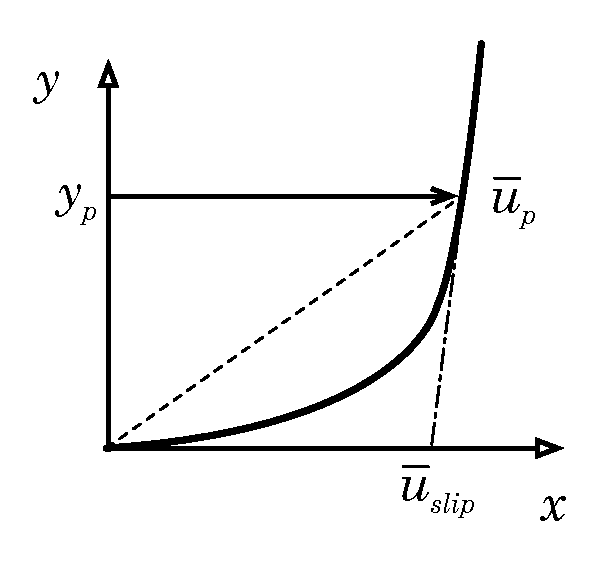
\includegraphics[width=5cm,clip]{wallfunc.eps}
\end{center}
\caption{壁面近傍の無次元速度プロファイル(\cite{kajishima:99:simulation}から転写)}
\label{fig:wall func}
\end{figure}


%%
\subsubsection{壁法則の適用}
%
\paragraph{発達した流れの場合}
チャネル流や円管内の発達流の場合,平均圧力勾配$\partial p^{\prime} / \partial x_i^{\prime}$と壁面摩擦力$\tau^{\prime}_w$が釣り合うので,\textbf{式(\ref{eq:friction velocity})}から摩擦速度がわかる.
第一格子点が対数則の範囲内であることが確認できれば,\textbf{式(\ref{eq:log-law log_e})}を利用できる.

%
\paragraph{流れの状況に応じて壁面摩擦が決まる場合}
一般的には,流れの様子により局所的な摩擦速度の大きさは異なるため,反復的に求める.
ある時点での$y_p^{\prime}$における$u_p^{\prime}$を与えて,関数として次の形を満たす$u_{\tau}^{\prime}$をニュートン反復により求める.

\begin{equation}
F(u_{\tau}^{\prime}) \,\equiv \, \frac{u_p^{\prime}}{u_{\tau}^{\prime}} - \frac{1}{\kappa}\mathrm{ln}\,\left( \frac{u_{\tau}^{\prime} \, y_p^{\prime}}{\nu} \right)\,-\,C \,=\,0
\label{eq:wall func newton}
\end{equation}

\noindent mを反復回数とすると,
\begin{equation}
{u_{\tau}^{\prime}}^{m+1} \,=\, {u_{\tau}^{\prime}}^{m} - \frac{F\left( {u_{\tau}^{\prime}}^{m} \right)}{F^{(1)} \left( {u_{\tau}^{\prime}}^{m} \right)}
\label{eq:newton iteration wall func}
\end{equation}

\noindent 対数則の場合には$F$の一階導関数は,
\begin{equation}
F^{(1)} \left( {u_{\tau}^{\prime}} \right) \,=\,
- \left( {\frac{u_p^{\prime}}{u_{\tau}^{\prime}} + \frac{1}{\kappa}} \right) \, \frac{1}{u_{\tau}^{\prime}}
\label{eq:derivative wall func}
\end{equation}

\noindent \textbf{式(\ref{eq:wall func newton})}$\sim$\textbf{(\ref{eq:derivative wall func})}から反復式を表すと,

\begin{equation} 
{u_{\tau}^{\prime}}^{\,m+1} \,=\, {u_{\tau}^{\prime}}^{\,m} + 
\frac{ 
\displaystyle{
\left\{
\frac{u_p^{\prime}}{{u_{\tau}^{\prime}}^{\,m}}
 - \frac{1}{\kappa} \, 
 \mathrm{ln}\,\left( \frac{y_p^{\prime} \, {u_{\tau}^{\prime}}^{\,m}} {\nu} \right) 
 \,-\, C \right\} \, 
 {u_{\tau}^{\prime}}^{\,m} }
}
{ \displaystyle{ \frac{u_p^{\prime}}{{u_{\tau}^{\prime}}^{\,m}} + \frac{1}{\kappa} }
}
\label{eq:newton iteration wall func}
\end{equation}


摩擦速度を無次元で表し$u_{\tau}\,=\,u_{\tau}^{\prime}/u_0^{\prime}$とすると,

\begin{equation} 
u_{\tau}^{\,m+1}
\, = \,
u_{\tau}^{\,m} + 
\frac{ 
\displaystyle{
\left\{ 
u_p^{+\,m} - \frac{1}{\kappa} \, 
 \mathrm{ln}\,\left( y_p^{+\,m} \right) \,-\, C \right\} \, u_{\tau}^{\,m} }
}
{ \displaystyle{ u_p^{+\,m} + \frac{1}{\kappa} }
}
\label{eq:newton iteration wall func ND}
\end{equation}

上記の手順により求めた$u_{\tau}^{\prime}$に対して,$y_p^{\prime}$が対数則の範囲にあるかどうかを判定し,壁法則を適用する.

%
\vspace{5mm}
\paragraph{摩擦速度求解のアルゴリズム}
与えられたセル近傍の速度から摩擦速度を求める手順は以下のようになる.

\begin{enumerate}
\item 反復の初期値を計算する.
\begin{equation}
\begin{array}{l}
\vspace{3mm}
\displaystyle{ \tau_w^0 \,=\, \frac{\tau_w^{\,\prime}}{\rho^{\prime} {u_0^{\prime}}^2} \,=\, \frac{1}{Re} \frac{\partial u}{\partial y} }\\
\vspace{3mm}
\displaystyle{ u_{\tau}^{\,0} \,=\, \frac{u_{\tau}^{\prime\,0}}{u_0^{\prime}} \,=\, \frac{1}{u_0^{\prime}} \sqrt{\frac{\tau_w^{\,\prime}}{\rho^{\prime}}}
\,=\, \sqrt{\frac{1}{Re} \frac{\partial u}{\partial y}} }\\
\vspace{3mm}
\displaystyle{ {y_p^+}^{\,0} \,=\, \frac{u_{\tau}^{\,0} \, u_0^{\prime} \, y_p^{\prime} }{\nu} }
\,=\, u_{\tau}^{\,0} \, y_p^{\prime} \, \frac{Re}{L^{\prime}}\\
\end{array}
\label{eq:initial iteration fric vel}
\end{equation}
ここで,$L^{\prime}$は代表長さ,$y_p^{\prime}=h^{\prime}/2$(バイナリボクセルの場合は,壁面から半セルの距離)である.
速度勾配は次の2つの候補がある.
\vspace{1mm}

\begin{indentation}{5zw}{0zw}

\begin{enumerate}
\item 壁面から半セルの距離にある速度定義点の速度の大きさで評価
\begin{equation}
\frac{\partial u}{\partial y}  \,=\, \frac{\Delta u}{\Delta y} \,=\, \frac{|u|}{h/2}
\label{eq:vel mag wall func}
\end{equation}

\item \textbf{図\ref{fig:wall func}}の$y_p$の位置での速度勾配を壁関数\textbf{(\ref{eq:log-law log_10})}から求める
\begin{equation}
\frac{\partial u}{\partial y}  \,=\, \frac{5.75}{y_p^+ \, \mathrm{ln}10}
\label{eq:dudy wall func}
\end{equation}

\end{enumerate}

\end{indentation}

\vspace{2mm}

\item Newton反復(常用対数を用いて)
\begin{equation} 
u_{\tau}^{\,m+1} \,=\, u_{\tau}^{\,m} + 
\frac{ \displaystyle{
\left\{ u_p^{+\,m} -  5.75 \, \mathrm{log_{10}}\,{y_p^+}^m \,-\, 5.5 \right\} \, u_{\tau}^{\,m} }
}{ \displaystyle{
u_p^{+\,m} + \frac{1}{\kappa} }
}
\label{eq:newton iteration wall func ND2}
\end{equation}

\vspace{2mm}
\item 収束判定
次式により収束判定を行う.
\begin{equation} 
\displaystyle{ \frac{|u_{\tau}^{\,m+1}-u_{\tau}^{\,m}|}{|u_{\tau}^{\,m}|} < \epsilon_2 \quad(=10^{-3}) }
\label{eq:newton iteration criteria}
\end{equation}

ここで,$u_{\tau}^{\,m+1}<\epsilon_2$の場合には,安定性のために$u_{\tau}^{\,m+1}=\epsilon_2$とする.
\vspace{2mm}

\item 更新\\
\begin{equation}
\begin{array}{l}
u_{\tau}^{\,m} \,=\, u_{\tau}^{\,m+1}\\
\vspace{2mm}
\displaystyle{ {y_p^+}^{\,m} \,=\, u_{\tau}^{\,m+1} \, y_p^{\prime} \, \frac{Re}{L^{\prime}} }\\
\end{array}
\label{eq:newton iteration wall func ND2}
\end{equation}
\vspace{2mm}

\item 上記を収束するまで繰り返す.反復上限を10回程度で抑えておく.
\end{enumerate}


%
\subsubsection{減衰関数を用いたすべりなし条件}

壁近傍ではGSで速度勾配があるため,SGS応力が生じる.しかし,壁面上では$\tau_{ij}=0$なので,これを打ち消す必要がある.
Smagorinskyモデルでは減衰関数$f_s$を導入し,渦粘性係数を補正する.

\begin{equation}
\nu_e \,=\, \left( Cs \,f_s \, \overline{\Delta} \right)^2 \left| \overline{D} \right|
\label{eq:nu-SGS modified}
\end{equation}

\noindent 減衰関数としてはvan Driest関数を用いる.

\begin{equation}
f_s \,=\, 1 - \mathrm{exp} \left( -\frac{y^+}{A^+} \right)
\label{eq:van-driest}
\end{equation}

\noindent $A^+$は無次元の定数で約25が用いられる.

すべりなし条件を用いる場合には,粘性底層からバッファ層にかけて,格子点が数点必要である.
この場合,粘性底層内では乱流応力は無視できるので,壁面摩擦応力$\tau_w^{\prime}$は次のように決められる.

\begin{equation}
\tau_w^{\prime} \,=\, \mu \left| \frac{\partial \overline{u^{\prime}}}{\partial y^{\prime}} \right|_{wall}
\label{eq:viscous layer stress}
\end{equation}

%
\subsection{壁法則から求めた壁面摩擦応力による粘性応力の置換}
壁面に接する流体セルの固体セルへの接平面上の壁面摩擦応力$\tau_w^{\prime}=\mu(\partial u^{\prime}/\partial y^{\prime})$は壁法則\textbf{(\ref{eq:friction velocity})}から求められる摩擦速度から$\tau_w^{\prime}\,=\, \rho^{\prime} {u_{\tau}^{\prime}}^2$として計算される.この壁面摩擦応力を粘性項の離散式に代入し境界条件とする.たとえば,z軸のマイナス方向に壁面がある場合,無次元形式で,

\begin{equation}
\frac{1}{Re} \frac{\partial}{\partial z} \left( \frac{\partial u}{\partial z} \right)
\,=\,
\frac{1}{h} \, \left( {\frac{1}{Re} \frac{\partial u}{\partial z}_t - \tau_{w,\,b} } \right)
\label{eq:replace wall shear stress}
\end{equation}


計算された摩擦速度から壁面摩擦応力を計算し,\textbf{式(\ref{eq:replace wall shear stress})}により境界条件を与える.固体セルに隣接する流体セルにおいて摩擦速度が求まると,固体に接する面上の応力は次式により計算される.

\begin{equation} 
\tau_w\,=\, u_{\tau}^2
\label{eq:wall stress from fric vel}
\end{equation}

\noindent しかしながら,複数の固体面に接するセルでは各方向同じ大きさの壁面摩擦応力となるし,軸方向に沿わない速度ベクトルの場合には過大評価になる可能性がある.そこで,速度ベクトルの方向成分を計算し,各方向へ射影する.つまり,\textbf{式(\ref{eq:wall stress from fric vel})}に用いる$u_{\tau}$を再定義する.

\begin{equation} 
\tau_{w,\,i} \,=\, {\left( u_{\tau} \frac{u_i}{|u|} \right)}^2
\label{eq:redefine of friction velocity}
\end{equation}



